\chapter{Configuration manuelle du projet (avancé)}
\label{sec-config-manual}

\renewcommand{\headrulewidth}{0.3pt}
\fancyhead[LE]{\thepage} \fancyhead[RE]{\nouppercase{\textbf{\leftmark}}}
\fancyhead[RO]{\thepage} \fancyhead[LO]{\nouppercase{\textbf{\rightmark}}}
\fancyfoot[L,C,R]{}

\setlength{\parindent}{0.35cm}

\minitoc
\newpage
% ================================================================

\alertinfo{La configuration du projet est désormais \textbf{automatisée} : lors d'un premier lancement normal, le plug-in détecte les sorties \cawaqs~et renseigne la configuration des géométries à votre place. La voie manuelle décrite dans ce chapitre est une \textbf{solution de repli} pour les utilisateurs avancés --- lorsque la détection automatique ne parvient pas à résoudre le projet, ou lorsqu'une configuration doit être construite ou ajustée à la main. Les nouveaux utilisateurs n'en ont pas besoin pour démarrer.}

La partie inférieure de la boîte de dialogue \gui{Settings} permet la configuration manuelle du plug-in. Les éléments suivants doivent être définis :
\begin{enumerate}
    \item un nom de projet ;

    \item les compartiments modélisés ;

    \item une configuration des maillages de couches SIG ;

    \item les répertoires de sorties de modélisation et d'observations\footnote{Les répertoires d'observations de débit et de piézométrie sont supposés se trouver dans le même répertoire parent.} si des points d'observation sont définis dans le projet.
\end{enumerate}

Le nom du projet servira à nommer un sous-dossier créé dans le répertoire de post-traitement. Les sorties graphiques de l'application \cwv~seront placées dans ce dossier de post-traitement.\\

La configuration des géométries peut aussi être importée depuis un fichier de configuration \json~(en cliquant sur \gui{Import a geometry configuration from a \json}) ou définie manuellement \textit{via} l'option \gui{Select resolutions from the current project}.

\alertinfo{Notez que toute configuration manuelle du projet et des géométries sera exportée au format \json~vers le répertoire de post-traitement à l'exécution de la boîte de dialogue \gui{Settings}.}

\section{Contenu du projet QGIS utilisé pour le traitement des résultats de simulation \cawaqs}
\label{sec-res-cawaqs}

\textbf{{Les \script{shapefiles} des maillages du modèle \cawaqs}}\\
Le projet QGIS utilisé pour le traitement des simulations avec l'utilitaire \cwv~doit contenir :
\begin{itemize}
    \item les maillages (résolutions) des compartiments au format \gui{shapefile} du modèle (référez-vous à la documentation \cawaqs\footnote{Terminologie des géométries \cawaqs. Pour plus d'informations sur les différents types de maillages, référez-vous à la documentation du modèle (\ie~guide utilisateur et guide technique), disponible sur le dépôt GitLab \href{https://gitlab.com/cawaqs/cawaqs}{https://gitlab.com/cawaqs/cawaqs}.} pour identifier les résolutions de sortie du compartiment \gui{WATBAL}). Les types de résolutions \cawaqs~à importer dans le projet SIG pour le traitement des sorties de modélisation dépendent des compartiments réellement modélisés ;

    \item les points d'observation des compartiments à définir dans l'extension \cwv.
\end{itemize}

\begin{table}[H]
    \centering
    \begin{tabular}{>{\raggedleft\arraybackslash}m{3cm}|>{\centering\arraybackslash}m{3.2cm}>{\centering\arraybackslash}m{3.2cm}>{\centering\arraybackslash}m{3.2cm}>{\centering\arraybackslash}m{3.2cm}}
        \hline
                                                                & \textbf{Compartiment de surface\newline(WATBAL)}                                                               & \textbf{Compartiment hydraulique \newline(HYD)} & \textbf{Compartiment non saturé \newline(NSAT)} & \textbf{Compartiment aquifère \newline(AQ)} \\
        \hline
        \textbf{Résolution \cawaqs}                             & Maille de surface unitaire (\texttt{ele\_bu})\footnotemark~ \newline ou maille de production (\texttt{Cprod}) & Élément de rivière (\texttt{ele\_musk})            & Grille de zone non saturée                     & Maillages de toutes les couches aquifères   \\
        \hline
        \textbf{Champs requis dans la table attributaire} & Identifiants de mailles                                                                                      & Identifiants SIG des éléments de rivière          & Identifiants de mailles                        & Identifiants absolus de mailles            \\
        \hline
    \end{tabular}
    \caption{Résolutions \cawaqs~pouvant être importées comme résolution de compartiment.}
    \label{tab-resolution_per_compartment}
\end{table}

\alertwarning{Les noms des couches SIG du projet correspondant aux aquifères doivent être identiques à ceux définis dans la configuration CaWaQS afin de garantir le bon comportement de l'application.}

\textbf{{Les \script{shapefiles} des points d'extraction}}\\

L'extraction des débits et charges hydrauliques simulés peut être réalisée aux points d'extraction. Deux types de points d'extraction peuvent être définis :
\begin{itemize}
    \item les points d'extraction simples, qui n'incluent pas de chronique de mesure ;

    \item les points d'observation, qui sont des points d'extraction disposant de données de mesure.
\end{itemize}

Les points d'extraction et d'observation sont contenus dans deux fichiers \script{shapefile} distincts dont les tables attributaires contiennent les champs listés dans la table \ref{tab_obs_extract}.

\vspace{8pt}

\renewcommand{\arraystretch}{1.5} % pour ajouter de l'espace entre les lignes
\newcolumntype{C}[1]{>{\centering\arraybackslash}p{#1}} \newcolumntype{C}[1]{>{\centering\arraybackslash}p{#1}}

\begin{table}[H]
    \begin{tabular}{|C{0.2\textwidth}|C{0.35\textwidth}|C{0.35\textwidth}|}
        \hline
        \textbf{TYPE DE POINT}& \textbf{CONTENU DE LA TABLE ATTRIBUTAIRE} & \textbf{SORTIES} \tabularnewline                    \hline
        \textbf{Point d'extraction}  &
        \begin{itemize}[leftmargin=*, itemsep=0.5ex]
            \item Nom du point
            \item Identifiant de la maille rattachée\footnote{\gui{GIS ID} en cas d'extraction dans le compartiment HYD, \gui{ABS ID} en cas d'extraction dans l'aquifère, champ optionnel}, identifiant de la couche aquifère (en cas d'extraction dans l'aquifère)\end{itemize} & \begin{itemize}[leftmargin=*, itemsep=0.5ex]\item Hydrogrammes et courbes piézométriques simulés au point d'extraction\end{itemize} \tabularnewline                     \hline
        \textbf{Point d'observation} &
        \begin{itemize}[leftmargin=*, itemsep=0.5ex]
            \item Nom du point
            \item Identifiant de la maille rattachée \footnotemark[\value{footnote}]
        \end{itemize} &
        \begin{itemize}[leftmargin=*, itemsep=0.5ex]
            \item Hydrogrammes et courbes piézométriques simulés et observés
            \item Critères objectifs comparant observations et simulations
        \end{itemize} \tabularnewline \hline
    \end{tabular}
    \caption{Structure des couches SIG des points d'extraction et sorties graphiques associées}
    \label{tab_obs_extract}
\end{table}

\vspace{8pt}

\alertwarning{Les \script{shapefiles} d'observation doivent être importés dans le projet et spécifiés dans la configuration \cwv~si les compartiments HYD et/ou AQ sont traités. Sans observations, l'extension ne sera pas fonctionnelle.}

\section{Configurer la géométrie du projet depuis un projet QGIS existant}
\label{sec_config_manuelle}

La configuration géométrique de l'application \cwv~peut être définie depuis un projet QGIS existant via la boîte de dialogue \gui{Application configuration from an existing project} dans la boîte de dialogue des paramètres de l'application.

La fenêtre est organisée en deux sections :
\begin{itemize}
    \item à gauche, les compartiments \cawaqs~sont listés (WATBAL, HYD, AQ, NSAT),

    \item à droite, les paramètres à définir sont listés pour produire les sorties graphiques (débit et piézométrie) aux points d'observation (points d'extraction avec observations) ou aux points d'extraction (sans observations).
\end{itemize}

Si les champs de configuration de l'application sont laissés vides, le compartiment concerné n'est pas inclus dans la configuration géométrique.\\

Les champs des compartiments sont configurés comme suit :\\

\noindent
\textbf{Le compartiment de surface (\gui{"WATBAL COMPARTMENT"}) :}

\vspace{0.5em}

\begin{minipage}[t]{0.45\textwidth}
    \begin{itemize}
        \item \gui{Surface resolution} : résolution de sortie du bilan hydrique de surface (CPROD ou elebu) ;
        \item \gui{cell id} : le numéro de colonne dans la table attributaire correspondant à l'identifiant de la maille ;
        \item \gui{cell area} : le numéro de colonne dans la table attributaire correspondant à l'aire de la maille (paramètre optionnel).
    \end{itemize}
\end{minipage}%
\hfill
\begin{minipage}[t]{0.45\textwidth}
    \centering
    \raisebox{\dimexpr-\height+\ht\strutbox}{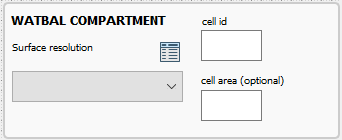
\includegraphics[
        width=0.8\linewidth
    ]{
        2_application_user_guide/fig/DialogSelectLayer_watbal.png
    }} \captionof{figure}{Champs de configuration du compartiment WATBAL}
\end{minipage}

\vspace{1em}
\textbf{Le compartiment hydraulique (\gui{HYD COMPARTMENT})}

\begin{minipage}[t]{0.45\textwidth}
    \begin{itemize}
        \item \gui{Hyd resolution} : nom de la résolution de sortie du compartiment \gui{HYD} (éléments de rivière) ;
        \item \gui{GIS Id} : le numéro de colonne dans la table attributaire correspondant à l'identifiant SIG des mailles
    \end{itemize}
\end{minipage}%
\hfill
\begin{minipage}[t]{0.45\textwidth}
    \centering
    \raisebox{\dimexpr-\height+\ht\strutbox}{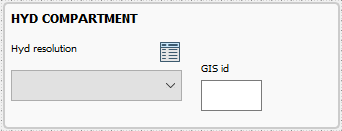
\includegraphics[
        width=0.8\linewidth
    ]{
    2_application_user_guide/fig/DialogSelectLayer_hyd.png
    }}
    \captionof{figure}{Champs de configuration du compartiment HYD}
\end{minipage}

\vspace{1em}
\textbf{Le compartiment non saturé (\gui{NSAT COMPARTMENT}) :}

\begin{minipage}[t]{0.45\textwidth}
    \begin{itemize}
        \item \gui{Unsatured zone resolution} : nom de la résolution de sortie du compartiment \gui{NSAT} ;
        \item \gui{cell id} : le numéro de colonne dans la table attributaire correspondant à l'identifiant de la maille.
    \end{itemize}
\end{minipage}%
\hfill
\begin{minipage}[t]{0.45\textwidth}
    \centering
    \raisebox{\dimexpr-\height+\ht\strutbox}{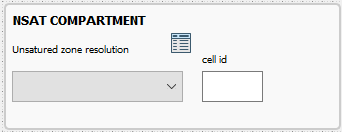
\includegraphics[
        width=0.8\linewidth
    ]{
    2_application_user_guide/fig/DialogSelectLayer_nsat.png
    }}
    \captionof{figure}{Champs de configuration du compartiment NSAT}
\end{minipage}

\vspace{1em}
\textbf{Le compartiment saturé (\gui{AQ COMPARTMENT})}

\begin{minipage}[t]{0.45\textwidth}
     \begin{itemize}
            \item \gui{Aquiferes resolutions} : les couches SIG constituant le maillage souterrain. La couche sélectionnée est ajoutée en cliquant sur \gui{Add}. Les couches doivent être ordonnées de la plus haute à la plus basse à l'aide des boutons \gui{up} et \gui{down}. Enfin, une couche peut être retirée de la liste en cliquant sur \gui{remove} ;
            \item \gui{cell id abs} : identifiant de la colonne de la table attributaire contenant l'identifiant absolu de la maille. Cet identifiant peut être homogène entre les couches SIG : dans ce cas, \gui{homogeneous ID ABS} doit être sélectionné. Sinon, cliquez sur \gui{heterogeneous ID ABS} pour ouvrir des boîtes de dialogue permettant de spécifier, pour chaque couche, la colonne contenant l'ID ABS des mailles (cf. Fig \ref{fig_id_abs_hetero}).
        \end{itemize}
\end{minipage}%
\hfill
\begin{minipage}[t]{0.45\textwidth}
    \centering
    \raisebox{\dimexpr-\height+\ht\strutbox}{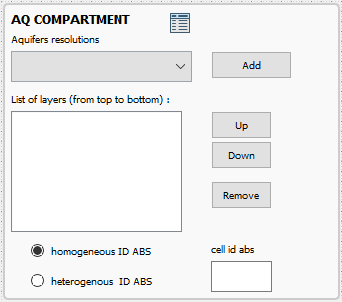
\includegraphics[
        width=0.8\linewidth
    ]{
    2_application_user_guide/fig/DialogSelectLayer_aq.png
    }}
    \captionof{figure}{Champs de configuration du compartiment AQ}
    \raisebox{\dimexpr-\height+\ht\strutbox}{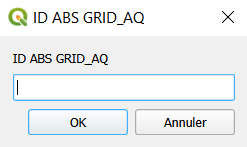
\includegraphics[
        width=0.5\linewidth
    ]{
2_application_user_guide/fig/DialogSelect_Layer_hetero_ID_ABS
    }}
    \label{fig_id_abs_hetero}
    \captionof{figure}{Fenêtre de sélection de l'identifiant du champ contenant l'\gui{ID ABS} dans la table attributaire dans le cas d'identifiants de champs hétérogènes entre les couches}
\end{minipage}



\alertwarning{Quelques points de vigilance :}
\begin{itemize}
    \item \textbf{L'identifiant de la première colonne d'une table attributaire commence à 0}. L'icône 
\includegraphics[height=0.45cm]{2_application_user_guide/fig/table.png} permet de visualiser les identifiants des champs listés dans la table attributaire de la résolution sélectionnée dans la liste déroulante ;
    \item le code (par ex. code BSS) d'un point d'observation doit être \textbf{unique} parmi tous les points d'observation ;
    \item La configuration géométrique des compartiments cochés dans la boîte de dialogue de paramétrage du projet doit être définie dans la boîte de dialogue de configuration des géométries.
\end{itemize}

\vspace{8pt}

\textbf{Points d'extraction - \gui{Hydrological and Hydrological plots}} \\
Les points d'extraction peuvent être de deux types :
\begin{itemize}
    \item[$\bullet$] les points d'extraction simples, qui permettent de visualiser les variables simulées en ces points ;
    \item[$\bullet$] les points d'observation, qui permettent de comparer les variables simulées aux données d'observation en ces points.
\end{itemize}



La configuration des points d'extraction nécessite de spécifier dans les champs \gui{GIS Layer} le nom de la couche du projet QGIS contenant les points d'observation et les points d'extraction selon le compartiment \cws~concerné. Les identifiants de champs à spécifier sont les suivants :
\vspace{8pt}

\begin{minipage}[t]{0.45\textwidth}
    \textbf{Points d'extraction du compartiment \gui{HYD}}
    \vspace{4pt}

     \underline{Points d'extraction}

    \begin{itemize}
        \item \gui{name} : nom du point d'observation ;
        \item \gui{ID GIS} : identifiant SIG du point d'observation auquel le point d'observation doit être rattaché (champ optionnel)
    \end{itemize}

    \vspace{2pt}
    \underline{Points d'observation}
    \begin{itemize}
        \item \gui{code} : code d'identification du point d'observation, doit être unique pour chaque point. Le fichier d'observation du point doit porter le même nom avec l'extension \script{.dat} ;
        \item les champs \gui{name} et \gui{ID GIS} sont également spécifiés pour la configuration des points d'observation
    \end{itemize}
    \vspace{8pt}
    \textbf{Points d'extraction du compartiment \gui{AQ}}
    \vspace{4pt}

     \underline{Points d'extraction}

    \begin{itemize}
        \item \gui{name} : nom du point d'observation ;
        \item \gui{ID LAYER} : identifiant de la couche aquifère
        \item \gui{ID GIS} : identifiant SIG du point d'observation auquel le point d'observation doit être rattaché (champ optionnel)
    \end{itemize}

    \vspace{2pt}
    \underline{Points d'observation}
    \begin{itemize}
        \item \gui{code} : code d'identification du point d'observation, doit être unique pour chaque point. Le fichier d'observation du point doit porter le même nom avec l'extension \script{.dat} ;
        \item les champs \gui{name} et \gui{ID GIS} sont également spécifiés pour la configuration des points d'observation
    \end{itemize}


\end{minipage}%
\hfill
\begin{minipage}[t]{0.45\textwidth}
    \centering
    \raisebox{\dimexpr-\height+\ht\strutbox}{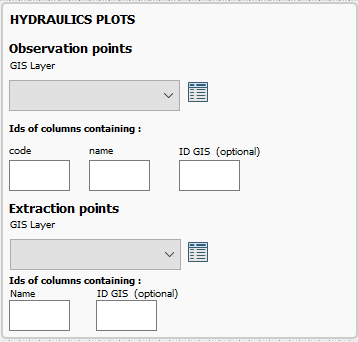
\includegraphics[
        width=0.9\linewidth
    ]{
    2_application_user_guide/fig/DialogSelectLayer_hyd_extraction.png
    }}
    \captionof{figure}{Champs de configuration des points d'extraction du compartiment \gui{HYD}}
    \vspace{4pt}
    \raisebox{\dimexpr-\height+\ht\strutbox}{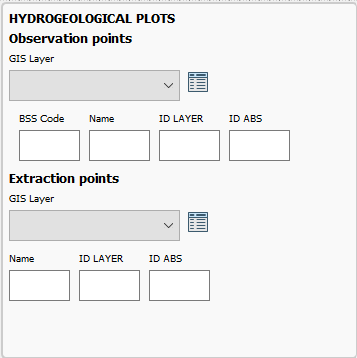
\includegraphics[
        width=0.9\linewidth
    ]{
    2_application_user_guide/fig/DialogSelectLayer_aq_extraction
    }}
    \label{fig_aq_extraction}
    \captionof{figure}{Champs de configuration des points d'extraction du compartiment \gui{AQ}}
\end{minipage}

\alertwarning{
Les points d'extraction doivent être contenus dans un fichier \script{.shp} différent de celui des points d'observation. Les points ne peuvent pas être contenus dans le même fichier s'ils sont extraits de deux compartiments différents.
}


\alertinfo{
Un enregistrement préalable du fichier de configuration des géométries peut être effectué en spécifiant un chemin de fichier dans le champ situé en bas à gauche de la boîte de dialogue. Ce fichier (\cfcod \ref{code_config_geom}) sera enregistré à l'exécution de la boîte de dialogue \gui{Settings} si le projet configuré n'existe pas encore dans le répertoire de post-traitement spécifié. Plusieurs configurations de projet peuvent être enregistrées dans le même répertoire de post-traitement, à condition qu'elles ne portent pas le même nom de projet. }



\section{Configurer les résolutions depuis un fichier de configuration \json}

La configuration géométrique des résolutions peut être spécifiée via un fichier \json~selon la structure suivante :

\begin{lstlisting}[language=json, caption={Contenu d'un fichier de configuration des géométries}, label={code_config_geom}]
{   // liste des compartiments CaWaQS a analyser (1 = AQ, 2 = HYD, 3 = WATBAL)
    "ids_compartment": [],

    "resolutionNames":
    {
        "1":
            [[""]], // liste des noms des maillages aquiferes dans le projet QGIS
        "2" :
            [[""]], // nom du maillage riviere dans le projet QGIS
        "3" :
            [[""]] // nom du maillage de surface dans le projet QGIS
        "4" :
            [[""]] // nom du maillage de zone non saturee dans le projet QGIS
        },
    "ids_col_cell": { // "id compartiment" : "numero de colonne de l'id de maille"
        "1" : "",  // "AQ id" : "numero de colonne de l'id absolu"
        "2" : "",  //"HYD id" : "numero de colonne de l'id SIG"
        "3" : ""   // "WATBAL id" : "numero de colonne de l'id de maille"
        },
    "obsNames": {
    // "id compartiment" : "nom du shp d'obs associe dans le projet QGIS"
        "1": "",
        "2" : ""
        },
    "obsIdsColCells": {
    // "id compartiment" : "numero de champ du code du point de mesure"
        "1": "",
        "2": ""
        },
    "obsIdsColNames": {
    // "id compartiment" : "numero de champ du nom du point de mesure"
        "1": "",
        "2" : ""
        },
    "obsIdsColLayers": {
    // "id compartiment" : "numero de champ de l'identifiant de couche aquifere"
        "1": "",
        "2" : null
        },
    "obsIdsCell": {
    // "id comp." : "numero de champ de l'id absolu ou sig de la maille rattachee a l'obs"
        "1" : "",
        "2" : null
    },
     "extNames": {
    // "id compartiment" : "nom du shp d'extraction associe dans le projet QGIS"
        "2": "",
        "1": ""
    },
    "extIdsColNames": {
    // "id compartiment" : "numero de champ contenant le nom du point d'extraction"
        "2": "",
        "1": ""
    },
    "extIdsColLayers": {
    // "id compartiment" : "numero de champ contenant l'identifiant de couche aquifere"
        "2": null,
        "1": ""
    },
    "extIdsColCells": {
    // "id compartiment" : "numero de champ contenant l'identifiant de maille"
        "1": "",
        "2": "",
    }
}
}
\end{lstlisting}
